% figures/K_2-3.tex

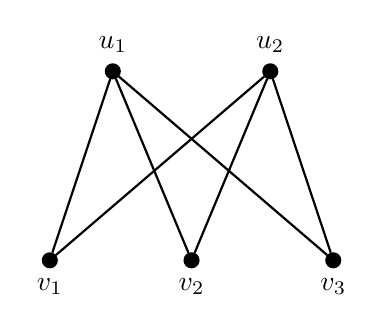
\begin{tikzpicture}[
    vertex/.style={circle, draw, fill=black, inner sep=0pt, minimum size=5pt},
    thick
]
    % Top partition (2 vertices)
    \node[vertex, label=above:{$u_1$}] (u1) at (0, 1.2) {};
    \node[vertex, label=above:{$u_2$}] (u2) at (2, 1.2) {};
    % Bottom partition (3 vertices)
    \node[vertex, label=below:{$v_1$}] (v1) at (-0.8, -1.2) {};
    \node[vertex, label=below:{$v_2$}] (v2) at (1, -1.2) {};
    \node[vertex, label=below:{$v_3$}] (v3) at (2.8, -1.2) {};
    % Edges
    \draw (u1) -- (v1);
    \draw (u1) -- (v2);
    \draw (u1) -- (v3);
    \draw (u2) -- (v1);
    \draw (u2) -- (v2);
    \draw (u2) -- (v3);
\end{tikzpicture}